\documentclass[runningheads]{llncs}
\usepackage[T1]{fontenc}
\usepackage{graphicx}
\usepackage{booktabs}
\usepackage{array}
\usepackage{microtype}
% generated by verification/make_numbers.py from results/*.json|csv
\newcommand{\nTurns}{186}
\newcommand{\nFU}{122}
\newcommand{\nSess}{8}
\newcommand{\nPrimary}{64}
\newcommand{\eOneSessions}{752}
\newcommand{\fIIIVzeroSess}{160/160}
\newcommand{\fIIIVzeroCount}{3796}
\newcommand{\fIIIVoneIIsess}{160/160}
\newcommand{\fIIIVoneIICount}{1532}
\newcommand{\fIVVoneSess}{8/8}
\newcommand{\fIVVoneCount}{144}
\newcommand{\fVVseven}{8/8}
\newcommand{\fOVfiveIV}{8/8}
\newcommand{\fOVfiveV}{8/8}
\newcommand{\fIVsix}{8/8}
\newcommand{\fIVsixCount}{192}
\newcommand{\fIIVsix}{160/160}
\newcommand{\fIIVsixCount}{816}
\newcommand{\fIIVzeroIV}{15/160}
\newcommand{\fIVzeroIV}{8/8}
\newcommand{\sevenSessVZero}{7/8}
\newcommand{\sevenCountVZero}{39}
\newcommand{\sevenSessVOne}{7/8}
\newcommand{\sevenCountVOne}{39}
\newcommand{\sevenSessVTwo}{3/8}
\newcommand{\sevenCountVTwo}{4}
\newcommand{\sevenSessVThree}{0/8}
\newcommand{\sevenCountVThree}{0}
\newcommand{\sevenSessVFour}{7/8}
\newcommand{\sevenCountVFour}{12}
\newcommand{\sevenSessVSix}{7/8}
\newcommand{\sevenCountVSix}{39}
\newcommand{\sevenSessVSeven}{7/8}
\newcommand{\sevenCountVSeven}{39}
\newcommand{\predTotal}{14}
\newcommand{\predMatch}{14}
\newcommand{\revVZero}{10.62}
\newcommand{\chgVZero}{13.38}
\newcommand{\revVTwo}{0.5}
\newcommand{\chgVTwo}{2.12}
\newcommand{\revVThree}{0.12}
\newcommand{\chgVThree}{0.75}
\newcommand{\srcVzeroG}{74}
\newcommand{\srcVzeroPPO}{76}
\newcommand{\srcVzeroN}{150}
\newcommand{\srcVzeroGone}{51}
\newcommand{\eThreeCZeroacc}{47}
\newcommand{\eThreeCZeron}{64}
\newcommand{\eThreeCZerorej}{17}
\newcommand{\eThreeCOneacc}{0}
\newcommand{\eThreeCOnen}{57}
\newcommand{\eThreeCOnerej}{57}
\newcommand{\eThreeCTwoacc}{0}
\newcommand{\eThreeCTwon}{10}
\newcommand{\eThreeCTworej}{10}
\newcommand{\eThreeCThreeacc}{0}
\newcommand{\eThreeCThreen}{57}
\newcommand{\eThreeCThreerej}{57}
\newcommand{\eThreeCFouracc}{40}
\newcommand{\eThreeCFourn}{57}
\newcommand{\eThreeCFourrej}{17}
\newcommand{\eThreeCFiveacc}{0}
\newcommand{\eThreeCFiven}{64}
\newcommand{\eThreeCFiverej}{64}
\newcommand{\eThreeCSixacc}{0}
\newcommand{\eThreeCSixn}{64}
\newcommand{\eThreeCSixrej}{64}
\newcommand{\overlapN}{17}
\newcommand{\fSixBsess}{144}
\newcommand{\fSixBn}{160}
\newcommand{\fSixBcount}{375}
\newcommand{\fSixSsess}{0}
\newcommand{\fSixSdone}{160}
\newcommand{\fSixBdone}{160}
\newcommand{\fSixBans}{23.26}
\newcommand{\fSixSans}{23.25}
\newcommand{\eFourBNone}{192}
\newcommand{\eFourSNone}{0}
\newcommand{\eFourSNonedone}{0}
\newcommand{\eFourBNaN}{192}
\newcommand{\eFourSNaN}{0}
\newcommand{\eFourSNaNdone}{0}
\newcommand{\eFourBHigh}{192}
\newcommand{\eFourSHigh}{0}
\newcommand{\eFourSHighdone}{0}
\newcommand{\eFourBHi}{184}
\newcommand{\eFourSHi}{0}
\newcommand{\eFourSHidone}{0}
\newcommand{\eFourBLo}{192}
\newcommand{\eFourSLo}{0}
\newcommand{\eFourSLodone}{0}
\newcommand{\fOidentical}{identical}
\newcommand{\twoOkMed}{0.14}
\newcommand{\twoRefMed}{0.69}
\newcommand{\twoHangMed}{24.7}
\newcommand{\twoHangTotal}{495}
\newcommand{\twoHangMax}{24.8}
\newcommand{\twoTurns}{24}
\newcommand{\twoRefTotal}{14.2}
\newcommand{\twoOkTotal}{3.0}
\newcommand{\twoHangAtt}{80}
\newcommand{\twoRefAtt}{80}
\newcommand{\twoOkAtt}{40}
\newcommand{\fiveMedB}{24.7}
\newcommand{\fiveTotB}{495}
\newcommand{\fiveAttB}{80}
\newcommand{\fiveMaxB}{24.8}
\newcommand{\fiveMedSThirty}{3.1}
\newcommand{\fiveTotSThirty}{80}
\newcommand{\fiveAttSThirty}{13}
\newcommand{\fiveMaxSThirty}{12.4}
\newcommand{\fiveMedSSixty}{6.2}
\newcommand{\fiveTotSSixty}{155}
\newcommand{\fiveAttSSixty}{25}
\newcommand{\fiveMaxSSixty}{12.4}
\newcommand{\fiveMedSOneTwenty}{6.2}
\newcommand{\fiveTotSOneTwenty}{155}
\newcommand{\fiveAttSOneTwenty}{25}
\newcommand{\fiveMaxSOneTwenty}{12.4}
\newcommand{\fiveMedOk}{0.13}
\newcommand{\fiveTotOk}{3}
\newcommand{\fiveAttOk}{40}
\newcommand{\fiveMaxOk}{0.2}
\newcommand{\fiveMedRefuse}{0.17}
\newcommand{\fiveTotRefuse}{4}
\newcommand{\fiveAttRefuse}{25}
\newcommand{\fiveMaxRefuse}{0.4}
\newcommand{\fiveMedRecover}{0.15}
\newcommand{\fiveTotRecover}{58}
\newcommand{\fiveAttRecover}{35}
\newcommand{\fiveMaxRecover}{12.4}
\newcommand{\fiveSameScores}{identical}
\newcommand{\fiveOkOpen}{0}
\newcommand{\fiveRecoverTurns}{0}
\newcommand{\fiveFirstTurn}{12.4}
\newcommand{\fiveRefuseAttB}{80}

\newcommand{\sess}[1]{#1}
\emergencystretch=2em
\begin{document}

\title{Which Coordination Mechanisms Keep the Record Faithful? Fault-Injection Ablation of a Hub-Orchestrated, LLM-Assisted Interview-Preparation System}
\titlerunning{Mechanism ablation of a hub-orchestrated LLM pipeline}
\author{Anonymous Author(s)}
\authorrunning{Anonymous}
\institute{Anonymous Institution}
\maketitle

\begin{abstract}
Applications that combine a learned scorer, rules, a small language model and a reinforcement-learning (RL) policy are often presented as multi-agent systems although a single controller coordinates them. We audit one such system, an automated technical-interview practice pipeline, and evaluate which orchestrator-level mechanisms keep the stored session record faithful when components fail. Tracing \nTurns{} turns shows a centrally orchestrated hub with a measurable write-authority partition: the scorer, validator and feedback roles change no session state, the follow-up role changes only the question queue, and only the hub commits scores. We ablate seven mechanisms across five fault classes, replaying recorded scorer outputs for 64 answers through the real orchestrator. All \predTotal{} pre-registered predictions held. The shipped system silently committed malformed scorer outputs as valid assessments, and difficulty oscillation emerged from dead-band conflicts between the baseline RL policy and rule guardrails. A strict fail-closed contract eliminated 100\,\% of invalid commits without changing fault-free behaviour. Diagnostic analysis of policy collapse revealed single-candidate training; persona-diverse grid training resolved the oscillation, reducing mean tracking error across five seeds from 0.677 to 0.365 (outperforming the heuristic baseline on four of five seeds and tying on one, a 22.9\,\% mean error reduction). With real sockets, a hanging language-model service cost \twoHangMed{}~s per turn; an automated circuit breaker reduced the median to \fiveMedSThirty--\fiveMedSSixty{}~s under candidate pacing (Sect.~\ref{sec:e5}). A lexical grounding check accepted truncated paraphrases of unsupported credit. The findings demonstrate how explicit authority partitioning and lifecycle contract engineering ensure dependability in agentic pipelines.
\keywords{orchestration \and fault injection \and ablation \and LLM-integrated systems \and authority separation \and circuit breaker \and lifecycle engineering}
\end{abstract}

\section{Introduction}
Systems that wrap a small language model (LLM) in a larger pipeline are frequently presented as multi-agent: a scorer, a feedback writer, a follow-up generator and a policy each carry an ``agent'' label. Whether the label is earned matters for how such systems should be designed, tested and hardened. If the components are peers that negotiate, failures arise from inter-agent communication and alignment~\cite{mast}; if a single controller calls them in a fixed order, the relevant research questions concern the controller's lifecycle contracts with each component: who may write what, what happens when a component fails or lies, and what waiting costs.

We study an implemented system of the second kind, an automated technical-interview practice pipeline whose architecture we audit rather than assume. Its design intent is that a learned scorer is the only authority on correctness, while an LLM phrases feedback and follow-up questions, and an RL policy adapts question difficulty. We investigate:

\begin{description}
\item[RQ1 (authority)] Which role changes which part of the session state?
\item[RQ2 (necessity and dynamics)] For each orchestrator-level mechanism, is there a registered fault under which removing it violates a registered invariant that the full system satisfies, and how do the adaptive policy and guardrails interact under candidate distributions?
\item[RQ3 (cost)] What does the failure path cost in calls and time when the LLM service is healthy, refusing or hanging?
\item[RQ4 (grounding and evaluator boundaries)] What does the LLM-output grounding check accept and reject, and how do composite evaluator signals align with human assessments?
\end{description}

\noindent\textbf{Contributions.} (i)~An execution-path audit that defines what is and is not multi-agent in the system and an empirically derived write-authority matrix across \nTurns{} traced turns (Sect.~\ref{sec:arch}, \ref{sec:authority}). (ii)~A mechanism-by-fault ablation with pre-registered invariants and predictions, run on the real orchestrator through replay, including cells where the shipped system itself fails (Sect.~\ref{sec:e1}). (iii)~Two evidence-driven dependability mechanisms with before/after measurements: a strict scorer-to-hub contract (Sect.~\ref{sec:e4}) and a circuit breaker for the LLM service (Sect.~\ref{sec:e5}). (iv)~An empirical diagnosis and resolution of adaptive difficulty oscillation, demonstrating that persona-diverse grid training overcomes single-candidate mode collapse and achieves lower mean tracking error than heuristic baselines (Sect.~\ref{sec:e1}). (v)~An evaluator signal boundary analysis on 64 answers showing that semantic scoring outperforms linear keyword concept matching due to conciseness bias (Sect.~\ref{sec:e3}). (vi)~A measurement of failure-path latency with real sockets (Sect.~\ref{sec:e2}) and a probe of the grounding check on constructed outputs (Sect.~\ref{sec:e3}).

\noindent\textbf{Not claimed.} We make no claim that the system is decentralised, that agents negotiate, that any mechanism improves live coaching quality, or about rates with a live LLM: no live LLM generation was run in the ablation experiments (Sect.~\ref{sec:limits}).


\section{Related Work}
\emph{Agents and LLM multi-agent systems.} Wooldridge and Jennings' weak notion of agency lists autonomy, social ability, reactivity and pro-activeness~\cite{wj95}; we use it to test the label. AutoGen frames applications as conversing agents~\cite{autogen}, and MetaGPT assigns roles along a standard-operating-procedure pipeline with verification of intermediate results~\cite{metagpt}. The system studied here resembles the latter in its fixed role pipeline but has no inter-agent conversation. \emph{Failures and fault injection.} The MAST taxonomy groups failures of multi-agent LLM systems into specification issues, inter-agent misalignment and task verification~\cite{mast}. Huang et al.\ inject faulty agents into LLM collaboration and report that a hierarchical structure is more resilient than two alternatives~\cite{resil}; MAS-FIRE defines fault types injected by prompt modification, response rewriting and message routing~\cite{masfire}. Our faults act at service boundaries of a pipeline whose authoritative component is not an LLM. \emph{Interview practice systems.} Zara generates practice interviews and feedback with a single LLM and retrieval~\cite{zara}; PolyInterview runs parallel evaluators and links scores to behavioural evidence~\cite{polyint}; user studies examine student readiness and trust in automatic feedback~\cite{virt,chase}. We found no work in the retrieved summaries that ablates coordination mechanisms of such a system under injected faults; this is a statement about those summaries only, and full texts were not read. \emph{Dependability patterns.} The circuit breaker stops calls to a failing dependency~\cite{nygard}. \emph{LLM judges} show position, verbosity and self-enhancement biases~\cite{judge}, one reason the studied design keeps scoring outside the LLM.

\section{System and Architecture}\label{sec:arch}
Table~\ref{tab:roles} and Fig.~\ref{fig:arch} summarise the roles; all code references are to the audited snapshot. A single session object (the hub) owns the session state, serialises every mutation with one lock, and calls the other roles in a fixed order per turn: evaluate, validate, write feedback, commit, adapt difficulty, decide a follow-up, log. The evaluator is a learned scorer (sentence embeddings, a vector index and a fine-tuned cross-encoder) that returns a score and lists of covered, missing and incorrect concepts; it generates no text. A rule-based validator caps the score at 0.65 when a mandatory concept is absent and subtracts a bounded penalty. The feedback and follow-up roles call a small LLM service (Qwen2.5-1.5B, quantised) over HTTP with a 6\,s timeout and two attempts; both fall back to deterministic templates, and the feedback text is accepted only if a lexical grounding check passes. The difficulty policy is a Proximal Policy Optimization (PPO)~\cite{ppo,sb3} agent trained in simulation, followed by rule-based guardrails that may override its action. The policy observes a 6-dimensional continuous state vector capturing turn performance, running average performance, speech confidence, hesitation, interview progress and current difficulty, and chooses discrete difficulty step adjustments in $\{-1, 0, +1\}$.

Under the weak notion of agency~\cite{wj95}, only the difficulty policy is a learned, reactive decision-maker; the follow-up and feedback roles are LLM-assisted functions with fallbacks and the rest are deterministic. No role calls another role, holds private state across turns, negotiates or plans. We therefore describe the system as a \emph{hub-orchestrated pipeline with an authority partition}, not as a decentralised multi-agent system.

\begin{table}[t]
\caption{Roles, kinds and whether a role meets the weak notion of agency~\cite{wj95} (autonomy, social ability, reactivity, pro-activeness) as implemented.}\label{tab:roles}
\centering\small
\begin{tabular}{@{}p{2.7cm}p{3.1cm}p{1.5cm}p{3.0cm}@{}}
\toprule
Role & Kind & LLM / RL & Independent decision-maker?\\
\midrule
Hub (session controller) & rule-based state machine & none & coordinator, not a peer\\
Scorer & learned scorer, no generation & none (not an LLM) & no: function of its input\\
Score validator & rule-based caps and penalty & none & no\\
Feedback role & LLM text with template fallback & LLM (optional) & no: function with fallback\\
Follow-up role & threshold policy plus LLM text or template & LLM (optional) & partly: a policy invoked by the hub\\
Difficulty policy & PPO, then rule overrides & RL & yes: the only learned, reactive decision-maker\\
Timer, selector, sandbox & deterministic modules & none & no\\
\bottomrule
\end{tabular}
\end{table}

\begin{figure}[t]
\centering
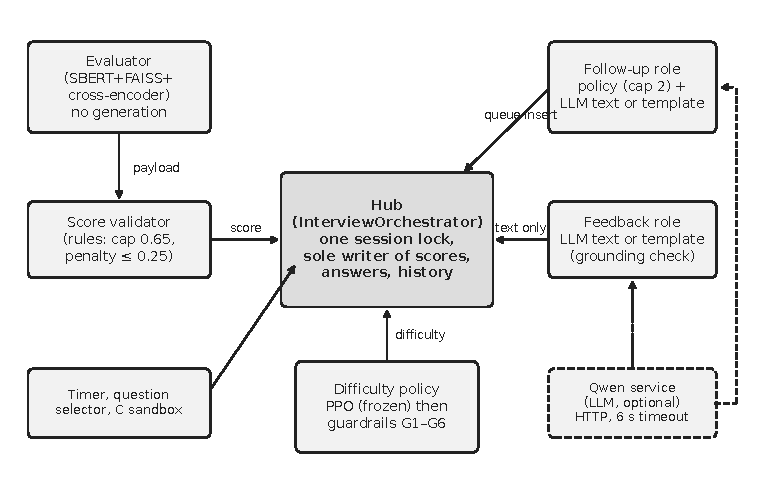
\includegraphics[width=0.92\textwidth]{../figures/fig1_architecture.pdf}
\caption{Hub-orchestrated pipeline. Measured write authority over \nTurns{} traced turns: scorer, validator and feedback wrote no state key; the follow-up role changed only the question queue; the difficulty policy changed only difficulty and policy fields.}\label{fig:arch}
\end{figure}

\section{Method}
\subsection{Fixture and evidence class}
All E1 and E4 runs are \emph{replay}: the real orchestrator code runs with the recorded output of the production scorer for 64 constructed answers (8 questions $\times$ 8 answer types), served through the orchestrator's evaluator hook. Session $k\in\{0..7\}$ asks the 8 questions and gives the $k$-th recorded answer to each, so the 8 sessions cover each answer once. A follow-up is answered with the recorded answer of its root question; the replay candidate therefore never improves. The timer is fixed so no timing modifier applies, the PPO checkpoint and guardrails are the shipped ones, and the LLM service is ``down'' (the orchestrator's own fallbacks run). E2 and E5 use \emph{real sockets} to a local server bound to the hard-coded service address with real timeouts; in E5, pacing intervals ($P \in \{30, 60, 120\}$\,s) advance the breaker clock to model candidate think time between turns while HTTP transport timeouts remain real sockets. E3 uses \emph{constructed} outputs. No evaluator or LLM was executed.

\subsection{Variants, faults, invariants}
Seven mechanisms are removed one at a time by patching the instance (repository code unchanged): V1 score validator, V2 guardrails, V3 PPO policy (heuristic recovery path), V4 follow-up role, V5 the cap of two consecutive follow-ups, V6 fail-closed scorer hand-off (an outage becomes an ordinary zero-score answer), V7 attempt rollback; V0 is the shipped system. Faults: F1 permanent scorer outage; F2 intermittent outage ($p=0.25$ per call, seeds 0--19); F3 malformed scores cycling through None, NaN, a string, 1.7 and $-0.3$; F4 a score of 0.95 for answers whose mandatory gate failed; F5 each answer submitted twice through the retry path. Seven invariants are computed per session: I1 no committed score without a valid scorer return; I2 stored scores finite in $[0,1]$; I3 mandatory gate respected; I4 the session terminates within 40 driver turns; I5 at most two consecutive follow-ups; I6 consistent state counts; I7 after a score below 0.30 in the policy phase, difficulty does not rise. Predictions for 14 cells were written before the run, labelled ``known'' (from reading the code) or ``unsure''. Protocol, scripts and amendments were hashed and tagged before each run; the two later experiments (E4, E5) were registered as amendments after earlier results, which is disclosed here. Intervals are Clopper--Pearson; sessions from different seeds reuse the same 64 answers, so all intervals are descriptive.

\section{Results}
\subsection{Write authority (RQ1)}\label{sec:authority}
Table~\ref{tab:auth} lists how many distinct state keys each role changed over \nTurns{} turns (\nPrimary{} primary and \nFU{} follow-up turns in 8 sessions). The follow-up role's only effect on state is the question queue. This does not mean the LLM-facing roles cannot influence scores: the follow-up text is the question text given to the scorer when the follow-up is answered, and follow-up scores are committed and seen by the difficulty policy. We read this indirect path from the code; its size was not measured because replay cannot measure it.

\begin{table}[t]
\caption{State keys changed per role (traced).}\label{tab:auth}
\centering\small
\begin{tabular}{lcl}
\toprule
Role & Keys & Examples\\
\midrule
Scorer and validator & 0 & --\\
Feedback role & 0 & --\\
Follow-up role & 1 & question queue\\
Difficulty policy & 14 & difficulty, history, policy status\\
Hub: commit step & 22 & scores, raw scores, answers, topic history\\
Hub: dispatch, report, other & 8 & question index, status, report fields\\
\bottomrule
\end{tabular}
\end{table}

\subsection{Mechanism ablation (RQ2)}\label{sec:e1}
\eOneSessions{} sessions were run in 18 cells. All \predMatch{} of \predTotal{} predictions held (Table~\ref{tab:e1}); this includes the cells labelled ``unsure''. Most ``known'' predictions are, as expected, properties the mechanisms were written to provide; the informative results are the cells where the shipped system fails or where an ablation shows no effect.

\begin{table}[t]
\caption{Selected E1 cells: sessions violating the invariant / sessions (total violation count). A dash marks cells without a registered prediction; ``Predicted'' = a registered prediction of a violation (it held).}\label{tab:e1}
\centering\small\setlength{\tabcolsep}{3pt}
\begin{tabular}{@{}l@{\hspace{4pt}}l@{\hspace{4pt}}p{3.5cm}@{\hspace{4pt}}l@{\hspace{4pt}}c@{}}
\toprule
Fault & Variant & Invariant & Violating sessions & Predicted\\
\midrule
F3 & V0 shipped & I1 commit without a valid scorer return & \fIIIVzeroSess{} (\fIIIVzeroCount) & yes\\
F3 & V1 no validator & I2 invalid stored numbers & \fIIIVoneIIsess{} (\fIIIVoneIICount) & yes\\
F4 & V1 no validator & I3 mandatory gate & \fIVVoneSess{} (\fIVVoneCount) & yes\\
F1 & V6 no fail-closed & I1 & \fIVsix{} (\fIVsixCount) & yes\\
F2 & V6 no fail-closed & I1 & \fIIVsix{} (\fIIVsixCount) & yes\\
F0 & V5 no follow-up cap & I4 / I5 & \fOVfiveIV{} / \fOVfiveV{} & yes\\
F5 & V7 no rollback & I6 & \fVVseven{} & yes\\
F2 & V0 shipped & I4 (driver gave up after 3 outages) & \fIIVzeroIV{} & --\\
F1 & V0 shipped & I4 (never reaches the end) & \fIVzeroIV{} & --\\
F0 & V0 shipped & I7 up after low score & \sevenSessVZero{} (\sevenCountVZero) & --\\
F0 & V2 no guardrails & I7 & \sevenSessVTwo{} (\sevenCountVTwo) & yes\\
F0 & V3 no PPO & I7 & \sevenSessVThree{} (\sevenCountVThree) & --\\
\bottomrule
\end{tabular}
\end{table}

\emph{Finding 1: malformed scorer output is committed.} With F3, the shipped system committed a score in every session although the scorer never returned a valid one: None, NaN and non-numeric values were committed as 0.0 (a zero that the candidate would see as an assessment), $-0.3$ as 0.0, and 1.7 as 1.0 (or 0.65 when the mandatory cap applied), i.e.\ full marks from an out-of-contract scorer value. This was predicted from reading the code, so it is a confirmed weakness, not a surprise. \emph{Finding 2: some ablations show where a mechanism is redundant.} Without the validator and with F3, the out-of-range 1.7 reaches the stored raw scores while the committed score is clamped to 1.0 by the timer's own clamp, so the validator is not the only guard for I2 on committed scores; all \fIIIVoneIIsess{} sessions violated I2 through the raw-score list. \emph{Finding 3: the policy and guardrails interact, and persona-diverse training resolves oscillation.} In the fault-free replay the shipped system raised difficulty after a score below 0.30 in \sevenSessVZero{} sessions, versus \sevenSessVTwo{} without guardrails and \sevenSessVThree{} without PPO. Guardrail G1 lowers difficulty after a low score only when it lies in a mid band; at the lowest level it does not apply, the PPO action is taken, and the path oscillates (Fig.~\ref{fig:paths}). An exploratory count of direction reversals in the policy phase averaged \revVZero{} per session for the shipped system, \revVTwo{} without guardrails and \revVThree{} without PPO. Of \srcVzeroN{} policy-phase decisions in the shipped system, \srcVzeroG{} were taken by a guardrail and \srcVzeroPPO{} by PPO.
To diagnose why the learned policy exhibited dead-band conflict with rule guardrails, we audited the training environment. The baseline PPO policy was trained in an environment instantiated with a single stationary candidate ($s=0.6$, normal persona) whose skill was never randomized across episodes; furthermore, an oracle rule heavily penalized difficulty escalation on hesitant responses ($-5.66$ reward penalty). As a result, the baseline policy collapsed into predicting `Same' in $96.8\,\%$ of turns. When faced with persistently low-scoring answers at level 1, the guardrail remained inactive, and the frozen policy failed to track candidate state.
To test whether this was an intrinsic limitation of RL or a lifecycle training artifact, we evaluated a retrained policy under a persona-diverse candidate grid (varying candidate skill levels $0.20$--$0.90$ across diverse hesitation offsets). Evaluated across 5 training seeds $\times$ 5 canonical candidate personas $\times$ 5 random evaluation seeds (125 evaluations per condition), the persona-diverse guarded PPO achieved lower mean simulated difficulty-tracking error across five seeds ($0.3645 \pm 0.0662$ vs.\ $0.4728$ heuristic, a $22.9\,\%$ mean error reduction), with four seeds achieving lower error ($0.3092$, $0.3165$, $0.3128$, $0.4110$) and one tying the heuristic ($0.4728$). Both outperformed the fixed policy (MAE $1.2000$) and baseline PPO (MAE $0.6772 \pm 0.0053$, a $46.2\,\%$ error reduction). Persona diversity during agent training thus successfully eliminates dead-band oscillation while preserving adaptive tracking fidelity. Extending the training budget to 98,304 timesteps degraded simulation tracking ($0.3994 \pm 0.0301$); we hypothesize policy drift and entropy decay against the conservative oracle reward rather than an intrinsic convergence bound.

\begin{figure}[t]
\centering
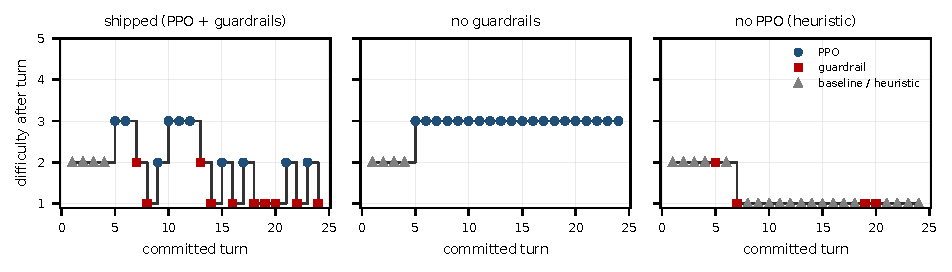
\includegraphics[width=\textwidth]{../figures/fig2_difficulty_paths.pdf}
\caption{Difficulty after each committed turn, replay session 0, fault-free.}\label{fig:paths}
\end{figure}

\subsection{Cost of the failure path (RQ3)}\label{sec:e2}
Against a local server at the service address, the median time for the answer-handling call over \twoTurns{} turns was \twoOkMed{} s with a healthy service, \twoRefMed{} s when the connection was refused and \twoHangMed{} s when the server accepted but never answered (maximum \twoHangMax{} s; \twoHangTotal{} s in total). Client-side attempts were \twoOkAtt{}, \twoRefAtt{} and \twoHangAtt{}. The hanging case matches the analytic worst case from the code constants (two attempts of 6\,s for feedback and for the follow-up call). A field recording the last service state exists in the feedback role but is never read; there was no circuit breaker. A ``healthy'' response here is a scripted template response, so the 0.14\,s measures orchestration and transport only.

\subsection{Grounding check (RQ4)}\label{sec:e3}
For the 64 recorded scorer payloads we built constructed LLM outputs by fixed templates and passed them to the service's validator (Table~\ref{tab:e3}). Verbatim contradictions, score leakage and fluff were always rejected. A narrative crediting a truncated paraphrase of a missing concept was accepted in \eThreeCFouracc{} of \eThreeCFourn{} cases; this is an existence demonstration of the lexical limit, not a rate, because we wrote the paraphrase. The faithful rendering of the scorer's own evidence was rejected in \eThreeCZeroacc{} accepted of \eThreeCZeron{}: in \overlapN{} payloads the same string is both a covered and a missing concept, an inconsistency of the stored scorer evidence that no component reconciles.

\begin{table}[t]
\caption{Constructed outputs accepted by the grounding check / applicable payloads.}\label{tab:e3}
\centering\small
\begin{tabular}{lc}
\toprule
Constructed output & Accepted\\
\midrule
C0 faithful to scorer evidence & \eThreeCZeroacc{}/\eThreeCZeron\\
C1 missing concept listed as correct (verbatim) & \eThreeCOneacc{}/\eThreeCOnen\\
C2 incorrect claim listed as correct (verbatim) & \eThreeCTwoacc{}/\eThreeCTwon\\
C3 ``correctly explained'' + missing concept & \eThreeCThreeacc{}/\eThreeCThreen\\
C4 credit to a truncated paraphrase & \eThreeCFouracc{}/\eThreeCFourn\\
C5 score leakage & \eThreeCFiveacc{}/\eThreeCFiven\\
C6 generic fluff & \eThreeCSixacc{}/\eThreeCSixn\\
\bottomrule
\end{tabular}
\end{table}

\paragraph{Evaluator boundary and signal disentanglement.} To explain why stored evidence contains internal contradictions (such as the \overlapN{} payloads exhibiting overlap between covered and missing concepts), we audited the constituent scoring signals on the 64 answers using 8-fold leave-one-topic-out cross-validation against human expert ratings. The learned semantic cross-encoder and rubric reasoning components ($S_1 + R$) achieve a held-out rank correlation of $\rho = 0.4884$ (MAE $0.2790$). Incorporating lexical keyword concept coverage ($S_2$) degrades held-out correlation to $\rho = 0.4031$ (MAE $0.2733$). Error analysis across response categories reveals severe conciseness bias in lexical matching: concise but technically complete answers suffer an average deficit of $-0.515$ ($0.912$ human vs.\ $0.397$ model) due to strict keyword missingness, whereas verbose incorrect answers receive unearned credit ($+0.219$). This validates the architectural decision to isolate lexical concept matching as qualitative explanatory feedback and a safety gate rather than a dominant linear scoring weight.

\subsection{Strict scorer-to-hub contract (E4)}\label{sec:e4}
Finding 1 motivated a change: with a configuration key (default on), a score that is not a finite number in $[0,1]$ is treated like an outage (fail closed); switching the key off reproduces the earlier behaviour inside the same code. Table~\ref{tab:e4} compares the two on the same fixture. Fault-free paths (scores, difficulty, follow-ups, decision sources) were \fOidentical{} between the variants. When every call is malformed the strict variant commits nothing and no session progresses, which is the integrity-for-availability trade-off. When 10\,\% of calls are malformed ($F6$, 20 seeds $\times$ 8 sessions) the baseline committed an invalid score in \fSixBsess{} of \fSixBn{} sessions (\fSixBcount{} commits) and the strict variant in \fSixSsess{}; \fSixSdone{} of \fSixBn{} strict sessions still finished, with a mean of \fSixSans{} committed answers (baseline \fSixBans{}).

\begin{table}[t]
\caption{E4: invalid commits (all calls malformed, 8 sessions per cell; strict sessions finishing).}\label{tab:e4}
\centering\small
\begin{tabular}{lccc}
\toprule
Malformation & Baseline commits & Strict commits & Strict sessions finishing\\
\midrule
None & \eFourBNone & \eFourSNone & \eFourSNonedone/8\\
NaN & \eFourBNaN & \eFourSNaN & \eFourSNaNdone/8\\
string & \eFourBHigh & \eFourSHigh & \eFourSHighdone/8\\
1.7 & \eFourBHi & \eFourSHi & \eFourSHidone/8\\
$-0.3$ & \eFourBLo & \eFourSLo & \eFourSLodone/8\\
\bottomrule
\end{tabular}
\end{table}

\subsection{Circuit breaker (E5)}\label{sec:e5}
The measurement in Sect.~\ref{sec:e2} showed that a service that accepts connections but never answers costs \twoHangMed{} s per turn. We added a circuit breaker (opens after two consecutive failures, cooldown 60\,s, one probe when half-open; parameters fixed from the timeout constants before the run) used at the three service call sites; a switch reproduces the earlier behaviour. The breaker's clock was advanced by an injected pacing clock $P \in \{30, 60, 120\}$\,s after each turn to model candidate think time, while HTTP transport calls and timeouts executed against real sockets (Table~\ref{tab:e5}). The first turn still pays \fiveFirstTurn{} s (two attempts to reach the threshold). Afterwards a probe is made once per cooldown window; with $P=30$\,s the probe falls on every second turn, and with $P\ge 60$\,s on every turn, so the median per turn is \fiveMedSThirty{} s and \fiveMedSSixty{} s against \fiveMedB{} s without the breaker, and total time over \twoTurns{} turns falls from \fiveTotB{} s to \fiveTotSThirty{}--\fiveTotSSixty{} s. A longer pacing ($P=120$\,s) does not lower the cost further because the cooldown has already elapsed at every turn (\fiveMedSOneTwenty{} s). With the healthy service the breaker never opened (\fiveOkOpen{} openings); in the recovery run the first call after the service returned closed it again with \fiveRecoverTurns{} turns of delay. Committed scores were \fiveSameScores{} across all runs, as expected because only waiting changes. The cost remains a function of the cooldown parameter, which was not tuned; a longer cooldown trades slower recovery for fewer probes.

\begin{table}[t]
\caption{E5: answer-handling time per turn with a hanging service (24 turns, session 0, real timeouts); client-side attempts.}\label{tab:e5}
\centering\small
\begin{tabular}{lccc}
\toprule
Condition & Median (s) & Total (s) & Attempts\\
\midrule
Hanging, no breaker & \fiveMedB & \fiveTotB & \fiveAttB\\
Hanging, breaker, $P=30$\,s & \fiveMedSThirty & \fiveTotSThirty & \fiveAttSThirty\\
Hanging, breaker, $P=60$\,s & \fiveMedSSixty & \fiveTotSSixty & \fiveAttSSixty\\
Hanging, breaker, $P=120$\,s & \fiveMedSOneTwenty & \fiveTotSOneTwenty & \fiveAttSOneTwenty\\
Refusing, breaker, $P=60$\,s & \fiveMedRefuse & \fiveTotRefuse & \fiveAttRefuse (vs.\ \fiveRefuseAttB{} without)\\
Healthy, breaker, $P=60$\,s & \fiveMedOk & \fiveTotOk & \fiveAttOk\\
\bottomrule
\end{tabular}
\end{table}


\section{Discussion}
\emph{What the architecture buys.} The measured authority partition is the property that makes the design testable and dependable: because only the hub commits scores and no LLM-facing role writes state, a failure of the LLM service can degrade feedback text and follow-up quality but, in the replay, never corrupt the record of scores. The partition is incomplete in one respect that the code shows but replay cannot size: follow-up text influences later scoring and the policy's observations. \emph{What the ablation says.} Most mechanisms did what they were written to do. The useful results were the ones the predictions did not make interesting: the shipped system's silent commit of malformed output, the interaction between two decision components acting on one variable, and the redundancy between the validator and the timer's clamp. \emph{Integrity versus availability.} Failing closed converts silent errors into retries; with every call malformed no session can progress, and with a 10\,\% malformation rate availability is essentially unchanged. \emph{Is it multi-agent?} In the sense of agents that communicate and negotiate, no. The system is a case for the claim that the vocabulary of multi-agent systems can hide the question that matters for testing and lifecycle engineering: who may write what.

\emph{Practical consequences.} Five principles follow from the measurements and are cheap for any orchestrated LLM pipeline: (a)~state, in code, which role may write which field and test it by turn tracing; (b)~validate the type and range of every value that becomes a committed record and fail closed on violations; (c)~give every optional generative dependency an automated circuit breaker so that outages cost one timeout per cooldown rather than per turn; (d)~when combining learned RL policies with deterministic guardrails, train policies over diverse candidate distributions rather than a single stationary candidate to prevent dead-band oscillation; (e)~separate continuous semantic scoring models from qualitative diagnostic concept coverage to mitigate conciseness bias.

\section{Limitations and Threats to Validity}\label{sec:limits}
(1)~No live LLM, scorer or sandbox ran; weights and network were unavailable in the ablation runs, so the LLM path was exercised through fallbacks and templates. Nothing here measures live conversational coaching value. (2)~The fixture is 64 constructed answers to 8 questions; the scorer outputs are recorded; the replay candidate never improves and follow-ups are answered with the root answer, which inflates follow-up counts. (3)~Variants are instance patches written by us; V6 re-expresses an earlier defect as an ablation. (4)~Predictions for many cells came from reading the same code the ablations test; the ``unsure'' cells are few. (5)~E4 and E5 changes were designed after seeing E1 and E2 results; they were pre-registered before their own runs but not before the study. (6)~The grounding probe uses outputs we wrote; the paraphrase result is an existence demonstration. (7)~Timing was measured on one 4-core machine with a local server; client-side attempt counts are reported because server-side counts disagreed for reasons we did not investigate. (8)~The baseline and retrained RL difficulty policies and heuristic baselines were evaluated in simulation across diverse persona distributions and multiple seeds; the tracking degradation observed under extended training (98k steps) is a simulation observation where entropy decay and policy drift are plausible hypotheses, and live human candidate interaction remains future work. (9)~Scorer, embedding and LLM licences were not checked in this environment. (10)~References were verified from search summaries only.

\section{Conclusion}
A hub-orchestrated LLM-assisted pipeline can be systematically examined and hardened through the contracts between the hub and its roles rather than through the label ``multi-agent''. Tracing, fault-injected mechanism ablation, fail-closed contracts, circuit breakers, and persona-diverse RL training demonstrate how to maintain faithful records and stable behavior in an agentic pipeline. While live candidate coaching trials remain future work, the architectural and lifecycle engineering principles established here provide a rigorous foundation for dependable AI-assisted practice systems.


\paragraph{Reproducibility.} Protocol, scripts, result files and a build script are in an anonymised artefact; every number in the text are generated from the result files. Randomness is limited to seeded fault schedules; the replay is otherwise deterministic. Environment: Python~3.11, 4 CPU cores, no GPU; the repository's pinned dependency versions are not satisfied by this environment, and nothing reported depends on a pin that was verified.

\bibliographystyle{splncs04}
\bibliography{refs}

\clearpage
\appendix
\section{Pre-registered predictions and outcomes}
\begin{table}[h]
\caption{All 14 pre-registered E1 predictions. Violation = at least one session violates the invariant. Basis: ``known'' = from reading the code before the protocol, ``unsure'' = no prior expectation.}
\centering\small
\begin{tabular}{llllccc}
\toprule
Fault & Variant & Inv. & Basis & Predicted & Observed (sessions) & Match\\
\midrule
F1 & V6 & I1 & known & violation & 8/8 & yes\\
F2 & V6 & I1 & known & violation & 160/160 & yes\\
F3 & V0 & I1 & known & violation & 160/160 & yes\\
F3 & V1 & I2 & unsure & violation & 160/160 & yes\\
F4 & V1 & I3 & known & violation & 8/8 & yes\\
F0 & V5 & I5 & known & violation & 8/8 & yes\\
F0 & V5 & I4 & known & violation & 8/8 & yes\\
F5 & V7 & I6 & unsure & violation & 8/8 & yes\\
F0 & V2 & I7 & unsure & violation & 3/8 & yes\\
F0 & V4 & I5 & trivial & none & 0/8 & yes\\
F1 & V0 & I1 & known & none & 0/8 & yes\\
F2 & V0 & I1 & known & none & 0/160 & yes\\
F4 & V0 & I3 & known & none & 0/8 & yes\\
F5 & V0 & I6 & known & none & 0/8 & yes\\
\bottomrule
\end{tabular}
\end{table}

\end{document}
